\documentclass[]{tufte-handout}

% ams
\usepackage{amssymb,amsmath}

\usepackage{ifxetex,ifluatex}
\usepackage{fixltx2e} % provides \textsubscript
\ifnum 0\ifxetex 1\fi\ifluatex 1\fi=0 % if pdftex
  \usepackage[T1]{fontenc}
  \usepackage[utf8]{inputenc}
\else % if luatex or xelatex
  \makeatletter
  \@ifpackageloaded{fontspec}{}{\usepackage{fontspec}}
  \makeatother
  \defaultfontfeatures{Ligatures=TeX,Scale=MatchLowercase}
  \makeatletter
  \@ifpackageloaded{soul}{
     \renewcommand\allcapsspacing[1]{{\addfontfeature{LetterSpace=15}#1}}
     \renewcommand\smallcapsspacing[1]{{\addfontfeature{LetterSpace=10}#1}}
   }{}
  \makeatother

\fi

% graphix
\usepackage{graphicx}
\setkeys{Gin}{width=\linewidth,totalheight=\textheight,keepaspectratio}

% booktabs
\usepackage{booktabs}

% url
\usepackage{url}

% hyperref
\usepackage{hyperref}

% units.
\usepackage{units}


\setcounter{secnumdepth}{-1}

% citations

% pandoc syntax highlighting

% longtable

% multiplecol
\usepackage{multicol}

% strikeout
\usepackage[normalem]{ulem}

% morefloats
\usepackage{morefloats}


% tightlist macro required by pandoc >= 1.14
\providecommand{\tightlist}{%
  \setlength{\itemsep}{0pt}\setlength{\parskip}{0pt}}

% title / author / date
\date{}


\begin{document}





\thispagestyle{empty}

\LARGE \emph{Test Property}\\
\Large \emph{Forest Management Plan}\\
\Large \emph{2020-01-07}

\begin{marginfigure}

{\centering 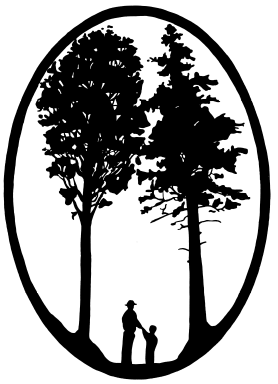
\includegraphics[width=0.3\linewidth,height=0.3\textheight]{C:/Users/Neal/projects/cruise/logo-small} 

}

\end{marginfigure}

\normalsize 

\begin{marginfigure}
\noindent \textit{\large Prepared by} 
\newline\indent Neal F. Maker and John D. Foppert  
\newline\indent Pekin Branch Forestry  
\newline\indent 1324 West County Road  
\newline\indent Calais, VT 05648  
\newline\indent (802) 229-9757  
\end{marginfigure}

\begin{marginfigure}
\noindent \textit{\large Owner}
\newline\indent Nobody  
\newline\indent PO Box 1
\indent 
\newline\indent Calais, VT 05648  
\end{marginfigure}

\begin{marginfigure}
\noindent \textit{\large Property}   
\newline\indent 7 acres and cabin   
\newline\indent Calais, VT  
\newline\indent SPAN 120-037-0000  
\newline\indent Map delineation based on VMP  
\newline\indent Photo(s) 1, 2  
\end{marginfigure}

\begin{marginfigure}
\noindent \textit{\large Effective date of plan}  
\newline\indent April 1, 2020  
\end{marginfigure}

\vspace{30pt} \indent This forest management plan is a blueprint for
responsible land stewardship. It is the result of a planning process
that incorporated an assessment of the history and current conditions on
the property, consideration of the various courses of future development
that the forest could follow, and discernment as to which outcomes best
suit my particular objectives.

\vspace{5pt} By signing below, I certify that I approve of---and agree
to manage my forestland according to---the following management plan. I
further certify that any of my forestland that is enrolled in Vermont's
Use Value Appraisal program is under active long-term forest management
in accordance with the state's minimum acceptable standards for forest
management. These standards include following Acceptable Management
Practices to maintain water quality on logging operations.

\vspace{38pt}

\noindent\rule{9cm}{0.4pt} \rule{.3cm}{0pt} \rule{4cm}{0.4pt}

\noindent Landowner \rule{7.7cm}{0pt} Date

\vspace{18pt}

\noindent\rule{9cm}{0.4pt} \rule{.3cm}{0pt} \rule{4cm}{0.4pt}

\noindent Landowner \rule{7.7cm}{0pt} Date

\vspace{18pt}

\noindent\rule{9cm}{0.4pt} \rule{.3cm}{0pt} \rule{4cm}{0.4pt}

\noindent Landowner \rule{7.7cm}{0pt} Date

\vspace{18pt}

\noindent\rule{9cm}{0.4pt} \rule{.3cm}{0pt} \rule{4cm}{0.4pt}

\noindent Landowner \rule{7.7cm}{0pt} Date

\vspace{24pt}

This forest management plan meets the standards promulgated by the
Vermont Department of Forests, Parks and Recreation as required for
eligibility in the Use Value Appraisal Program.

\vspace{22pt}

\noindent\rule{9cm}{0.4pt} \rule{.3cm}{0pt} \rule{4cm}{0.4pt}

\noindent County Forester \rule{7cm}{0pt} Date

\pagebreak

\section{Introduction}\label{introduction}

This plan Covers the ten year period from 2020 to 2029. It lays out the
near- and medium-term actions that should guide the development of the
Test Forest. It also qualifies the property for Use Value Appraisal
(UVA) and commensurate reduction in property taxes.\footnote{Further
  information about UVA and current valuations can be found at the
  Vermont Tax Department's website:
  \url{https://tax.vermont.gov/property-owners/current-use}.
  \vspace{20pt}} Owners participating in the Use Value Appraisal program
are obliged to manage their property according to the plan and to make
any reasonable investments for improvement that the plan
recommends.\footnote{UVA management plan standards are determined by the
  Department of Forests, Parks, \& Recreation and are available at
  \url{https://fpr.vermont.gov/forest/your_woods/use_value_appraisal} or
  through a County Forester.} Its recommendations were developed in
accordance with the principles and practices of scientifically sound
forestry, as described in the relevant management guidelines, textbooks
and academic journals.

\section{Property Description}\label{property-description}

Some 79 percent of the 7 acre Test property is productive forestland
that will be managed according to this plan. Its elevations range from
100 to 300 feet above mean sea level. There is some water on the
property. Like all parcels, there are boundaries. Soils, forest health,
and other pertinent topics are discussed in the individual stand area
descriptions that follow.

\section{Principles, Goals \& Strategies For Forest
Management}\label{principles-goals-strategies-for-forest-management}

\subsection{Wood production and timber
management}\label{wood-production-and-timber-management}

The forest should be able to sustainably provide a reliable supply of
fuelwood, fencing and building materials, and valuable, high quality
timber, either as sources of revenue or for consumption or utilization
directly on the farm or in the community. Long-term value growth is
provided by maintaining full site occupancy with healthy trees capable
of producing high quality sawtimber and veneer. Tree species which yield
sought-after, high-value wood shall be promoted within each stand or,
when regenerating within a stand, attention shall be paid to providing
the conditions which favor the establishment of those species. At a
property-wide scale, a variety of species shall be maintained to provide
opportunities to exploit future market opportunities and as a hedge
against species-specific market depreciation. Among desired species,
additional preference shall be given to individual trees of sufficient
vigor and grade-potential for strong future value growth. Consideration
of economic efficiency should inform the timing and coordination of
infrastructure investments and stand maintenance, improvement and
harvest operations.

\section{Stand Descriptions \& Management
Recommendations}\label{stand-descriptions-management-recommendations}

\begin{marginfigure}
\noindent \textit{\LARGE Management Schedule}
\vspace{10pt}

\noindent \textit{\large 2022}

\begin{itemize}
  \item Area 1: Group selection harvest  
\end{itemize}

\vspace{10pt}  
\noindent \textit{\large 2029}  

\begin{itemize}
  \item Reinventory property
\end{itemize}
\end{marginfigure}

Presented below are detailed stand-by-stand descriptions of the forest,
the long-term structural, compositional and functional goals for each
stand, and the near-term silvicultural treatments or management
activities that have been prescribed to advance each stand toward those
goals. The data presented in the following pages was obtained from a
field examination of the property in July of 2019. General conditions
were assessed qualitatively in conjunction with quantitative sampling.
Observational notes and sample summary statistics together provide the
basis for the area descriptions and management recommendations. All
sampling was done using a systematic sample and variable radius plots.
In stands with uneven-aged structures, all trees 6" dbh and larger were
measured in each plot. In stands with even-aged structures, all
main-canopy trees were measured in each plot.

When contractors are used to implement silvicultural prescriptions, they
should be highly skilled, properly equipped, fully insured, and closely
supervised. A professional forester should prepare and administer
commercial treatments, and logging operations should be timed to
coincide with favorable weather conditions (working on wet soils only
when they are frozen, for instance) and favorable timber markets. Use
Value Appraisal program guidelines allow any management activities
prescribed in this plan to be carried out up to three years before or
after the date indicated. Landowners in the Use Value Appraisal program
must file a Forest Management Activity Report with the County Forester
by February 1\textsuperscript{st} if any commercial logging occurred in
the previous year.

The property should be reinventoried in 2029 and the findings brought to
bear on a reassessment of the goals and strategies proposed in this
plan, leading to a formal management plan update. At any point over the
course of this management period, this plan may be updated to
incorporate new information and to reflect any new thoughts, concerns or
considerations on the part of the family or the foresters helping to
manage their land.

\newpage

\section{Area 1}\label{area-1}

Mixedwood\\
\noindent 5.50 legal acres \textbar{} 5.00 measured acres

\subsection{Site-specific information}\label{site-specific-information}

\begin{quote}
\begin{itemize}
\tightlist
\item
  \textbf{Soils:}\\
  \indent\indent  \textbf{Glover-Vershire complex} (shallow to
  moderately deep, excessively drained to well drained, loose, very
  rocky glacial tills on summits, shoulders, and backslopes)
\end{itemize}
\end{quote}

\begin{quote}
\begin{itemize}
\tightlist
\item
  \textbf{Site Class:}\\
  \vspace{2pt} II (determined from soil mapping and field assessment)
\end{itemize}
\end{quote}

\begin{quote}
\begin{itemize}
\tightlist
\item
  \textbf{Access:}\\
  \vspace{2pt} Less than 1 mile
\end{itemize}
\end{quote}

\begin{quote}
\begin{itemize}
\tightlist
\item
  \textbf{Stand history:}\\
  \vspace{2pt} invented
\end{itemize}
\end{quote}

\subsection{Current forest
information}\label{current-forest-information}

\begin{quote}
\begin{itemize}
\tightlist
\item
  \textbf{Age Class Structure:}\\
  \vspace{2pt} Uneven-aged\\

  \begin{marginfigure}
  \includegraphics{fmp-vt_files/figure-latex/unnamed-chunk-2-1} \caption[Distributions are approximated with kernel density estimation]{Distributions are approximated with kernel density estimation. Common species are those that account for at least 8 percent of the total stocking and areas under each curve represent species basal areas.}\label{fig:unnamed-chunk-2}
  \end{marginfigure}
\end{itemize}
\end{quote}

\begin{quote}
\begin{itemize}
\tightlist
\item
  \textbf{Species (\% stocking):}\\
  \vspace{2pt} hard maple (50\%), hemlock (50\%)
\end{itemize}
\end{quote}

\begin{quote}
\begin{itemize}
\tightlist
\item
  \textbf{Regeneration:}\\
  \vspace{2pt} none
\end{itemize}
\end{quote}

\begin{quote}
\begin{itemize}
\tightlist
\item
  \textbf{Forest health:}\\
  \vspace{2pt} awesome
\end{itemize}
\end{quote}

\begin{quote}
\begin{itemize}
\tightlist
\item
  \textbf{Size class structure (\%BA):}\\
  \vspace{2pt} \indent 6-10": 0\% \textbar{} 11-16": 50\% \textbar{}
  17-22": 50\% \textbar{} 23"+ : 0\%
\end{itemize}
\end{quote}

\subsection{Inventory information}\label{inventory-information}

\begin{quote}
\begin{itemize}
\tightlist
\item
  1 points, 10 BAF, July, 2019
\end{itemize}
\end{quote}

\begin{figure}
\includegraphics{fmp-vt_files/figure-latex/unnamed-chunk-5-1} \caption[Points represent individual plots]{Points represent individual plots. Asterisk represnts stand average. Radial lines are quadratic stand diameters.}\label{fig:unnamed-chunk-5}
\end{figure}

\begin{table}

\caption{\label{tab:unnamed-chunk-6}Measures of stocking for all live trees (total) and acceptable growing stock.}
\centering
\begin{tabular}[t]{lrr}
\toprule
  & Total & Acceptable\\
\midrule
Basal area (sqft/ac) & 120 & 60\\
QSD (in) & 6 & 6\\
Stems/ac & 528 & 264\\
\bottomrule
\end{tabular}
\end{table}

\subsection{Long-term management
system}\label{long-term-management-system}

\textbf{Even-aged management}\footnote{Leak, W.B., M.Yamasaki, and R.
  Holleran. 2014. Silvicultural Guide for Northern Hardwoods in the
  Northeast. USDA For. Serv. Gen.~Tech. Rep.~NRS-132.}

\subsection{Silvicultural
prescription}\label{silvicultural-prescription}

\textbf{Shelterwood establishment}\footnote{Leak, W.B., M.Yamasaki, and
  R. Holleran. 2014. Silvicultural Guide for Northern Hardwoods in the
  Northeast. USDA For. Serv. Gen.~Tech. Rep.~NRS-132.}\\
\textbf{Year:} 2022

\newpage



\end{document}
